\section{Model Inversion Attacks}

\subsection{MIFace}

MIFace (Model Inversion Face Attack), derin öğrenme modellerine karşı yapılan bir model inversion saldırısı türüdür. MIFace, yüz tanıma modellerinin çıktıları kullanılarak, modelin öğrendiği orijinal yüz resimlerini yeniden yapılandırmayı hedefler. Bu saldırılar, modelin eğitildiği gizli verileri açığa çıkarabilir ve böylece kullanıcı gizliliğini tehlikeye sokabilir.

MIFace saldırısı, bir yüz tanıma modelinin ara katman çıktıları veya sınıflandırma skorları gibi bilgilerden yararlanarak, modelin öğrendiği yüz görüntülerini yeniden yapılandırmayı amaçlar. Saldırgan, modelin her bir yüz için verdiği sınıflandırma skorları veya özellik vektörleri (feature vector) üzerinde analiz yapar. Modelin bu özellikleri kullanılarak, belirli bir bireyin yüzü yeniden oluşturulur. Yani modelin öğrendiği bilgiler tersine mühendislikle tekrar elde edilir.

\subsubsection{Python Kodu}

\begin{lstlisting}[language=Python]
from art.estimators.classification import KerasClassifier
from art.attacks.inference.model_inversion.mi_face import MIFace
tf.compat.v1.disable_eager_execution()

attack = MIFace(classifier, max_iter=10000, threshold=1.0)
infer_avg = attack.infer(avg, y)
\end{lstlisting}

\begin{figure}[h]
    \centering
    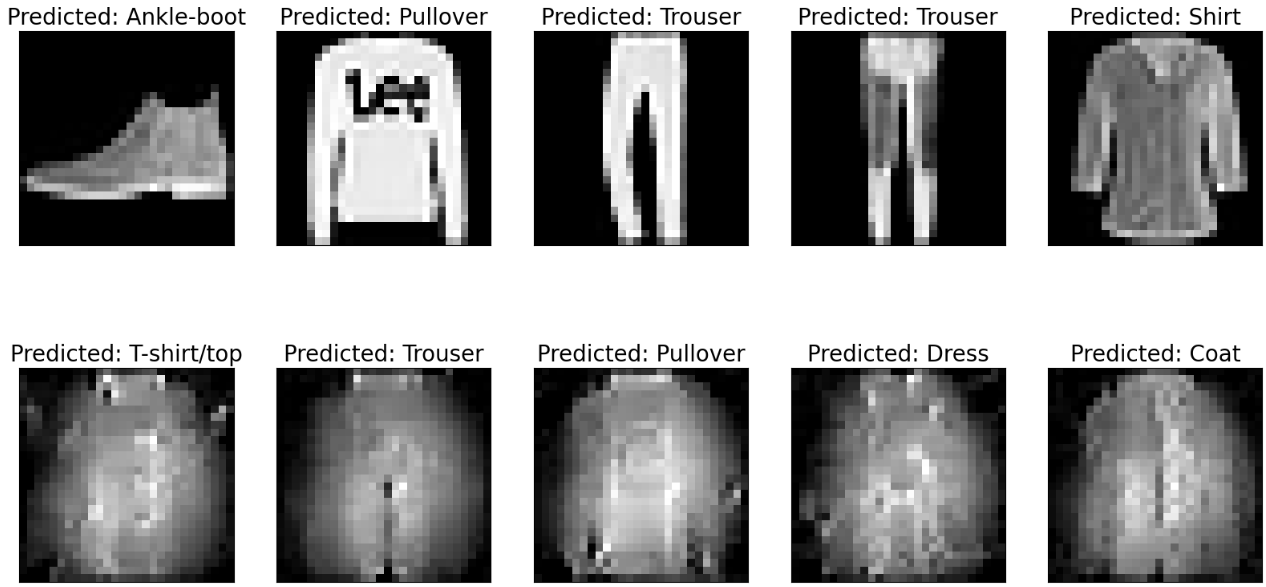
\includegraphics[width=1\textwidth]{images/miface_results.png}
    \caption{}
\end{figure}

\newpage